\documentclass[12pt,twoside,english,a4paper]{article}
%
\usepackage{etex}
% ----------- Packages ---------------------------------------------
\usepackage{ifthen}                % if then else Abfragen
% Boolesche Variable:
%  True  = Fette Gleichungsvariablen italic (kursiv)
%  False = Fette Gleichungsvariablen roman (gerade)
\newboolean{boldeqnitalic}
\setboolean{boldeqnitalic}{true} 

%\usepackage{german}
%\usepackage{ngerman}              % Neudeutsch
%\usepackage{showkeys}
%\usepackage{draftcopy}
\usepackage{caption}
\usepackage[latin1]{inputenc}
\usepackage[intlimits] {amsmath}   % muss for defjs# stehen
\usepackage{graphicx}
\usepackage{psfrag}
% \usepackage[usenames]{color}
%\usepackage[xdvi]{color}
\usepackage{ifthen}
\usepackage{fancyhdr}
\usepackage{rotating}
\usepackage{multirow}
\usepackage{booktabs}              % Dicke Tabellenlinien
\usepackage{amssymb}
\usepackage{amsbsy}
\usepackage{bm}                    % fette Schrift in Formeln
\usepackage{bbm}
\usepackage{babel}
\usepackage{theorem}
\usepackage{upgreek}  % gerade (roman) griechische Buchstaben z.B. \upalpha
\usepackage{pifont}   % zusaetzliche Schriften, z.B. eingekreiste Zahlen
\usepackage[active]{srcltx}   % aktive suche im xdv
\usepackage{subcaption}

% Zusaetzliche Schriften --- Anfang
% \usepackage[T1]{fontenc}
\usepackage{suetterl}  % Suetterlin Schrift
\newfont{\suetdbl}{suet14 scaled 2000}  % Suetterlin skaliert um Faktor 2,000

\usepackage{yfonts}  % altdeutsche Schrifte und Initialen
% nicht oldgerm verwenden, da 'yfonts' T1-encoding haben
\newfont{\gothdbl}{ygoth scaled 2000} 
\newfont{\frakdbl}{yfrak scaled 2000}
\newfont{\swabdbl}{yswab scaled 2000}
% Zusaetliche Schriften --- Ende


% Korrekturfunktionen --- Anfang
\usepackage[normalem]{ulem}  % zusaetzliche Unterstreichungsformen wie z.B.:
                             %  \uline \uuline \uwave \sout \xout
                             % Option 'normalem' deaktiviert die 
                             % Hervorhebung durch Unterstreichen
\usepackage[textsize=footnotesize,textwidth=1.7cm]{todonotes}
\setlength{\marginparwidth}{6cm}
\newcommand{\Crem}[1]{\textcolor{red}{\sout{#1}}}
\newcommand{\Cadd}[1]{\textcolor{blue}{\uline{#1}}}
\newcommand{\Cmod}[1]{\textcolor{green}{\dashuline{#1}}}
% Korrekturfunktionen -- Ende

\usepackage{defjs3}                % eigene Definitionen  
\newcommand{\cb}[1]{\overline{{\cal #1}}}   
\newcommand{\cbb}[1]{\boldsymbol{\overline{{\cal #1}}}}   


%\usepackage[latin1]{inputenc}
%
%-------------------------------------------------------------------
%\definecolor{mygrey}{gray}{0.75}
%
% --------- References Packages ----------------------------------------
\usepackage[authoryear]{natbib}
\bibpunct{[}{]}{,}{a}{}{;}
% Use the command \bibpunct with one optional and 6 mandatory arguments:
%    1. the opening bracket symbol, default = (
%    2. the closing bracket symbol, default = )
%    3. the punctuation between multiple citations, default = ;
%    4. the letter `n' for numerical style, or `s' for numerical
%       superscript style, any other letter for author-year,
%       default = author-year;
%    5. the punctuation that comes between the author names and the year
%    6. the punctuation that comes between years or numbers when
%       common author lists are suppressed (default = ,);
%
% --------- Seitenlayout -----------------------------------------------
\sloppy
\oddsidemargin   0.30cm            % linker Rand ungerade Seiten
\evensidemargin  0.30cm            % linker Rand gerade Seiten (twoside)
\topmargin       0.15cm            % OK Blatt - OK Kopfzeile
\topmargin      -1.35cm            % OK Blatt - OK Kopfzeile bei PS
\headheight      0.15cm            % Hhe der Kopfzeile
\headsep         0.70cm            % UK Kopfzeile - OK Rumpf
\topskip         0.60cm            % OK Rumpf - UK Textzeile
\textheight     24.50cm            % Texthhe
\textwidth      16.00cm            % Textbreite
\footskip        1.00cm            % Uk Rumpf - UK Fu{\'a}zeile
\fboxsep.3cm                       % Rahmenaufweitung 0.3cm
\setlength{\parindent}{0.0cm}      % Einzug 1. Zeile eines Absatzes
\setlength{\parskip}{1.ex}         % Abstand zweier Abs"atze
\setcounter{secnumdepth}{4}        % Tiefe der section Nummern
%
% -------- Kopfzeilen -------------------------------------------------
\setlength{\headheight}{14pt}
\pagestyle{fancy}
\renewcommand{\MakeUppercase}[1]{#1}    % Kopfzeilen nicht in gross
\fancyhead{}                            % Kopfzeile
\fancyhead[re] {\thepage}
\fancyhead[ro] {\thepage}
\fancyhead[ce] {\slshape 
AceGen and AceFEM integration of linear truss elements
}
\fancyhead[co] {\slshape  Max Bubendey, Sascha Maassen, J\"org Schr\"oder}
\fancyfoot{}                            % Fusszeile
%\fancyfoot[c]{\sffamily\small Version vom \today}
\fancypagestyle{plain}{%
  \fancyhead{}%
  \fancyfoot[c]{\sffamily\thepage}%
  \renewcommand{\headrulewidth}{0pt}%
}
\makeatletter                           % Leere Fuellseiten
\def\cleardoublepage{\clearpage\if@twoside \ifodd\c@page\else
  \hbox{}
  \vspace*{\fill}
  \thispagestyle{empty}
  \newpage
  \if@twocolumn\hbox{}\newpage\fi\fi\fi}
\makeatother
%\renewcommand{\chaptermark}[1]{\markboth {\chaptername\ \thechapter.\ #1}{}}
%\renewcommand{\sectionmark}[1]{\markright{\thesection\ #1}}
%
% ----------- Einbinden von Gleitobjektion ---------------------------
\setcounter{topnumber}{10}
\setcounter{bottomnumber}{10}
\setcounter{totalnumber}{10}
\renewcommand{\topfraction}{1.}
\renewcommand{\bottomfraction}{1.}
\renewcommand{\textfraction}{0.}
%
%----------- Trennungsvorgaben -------------------------------------
%\hyphenation{Span-nungs}
%\hyphenation{Ver-zer-rungs}
%
%------------ neue Definitionen ------------------------------------
%\newcommand{\IS}{{\rm\kern.24em         %fourth order Eshelby tensor
%   \vrule width.02em height1.4ex depth-.05ex
%   \kern-.26em S}}
% \newcommand{\M}{\mathbb{M}}
%-------------------------------------------------------------------
\begin{document}
\unitlength1.0cm
\frenchspacing
%
%========================================================================
%          ***  First Page of Paper  ***
%========================================================================
\thispagestyle{empty}

% \ce{{\Large UNIVERSITY OF DUISBURG ESSEN}
% \phantom{x}
% {\large CAMPUS ESSEN}}

\phantom{X\hfill X}

\unitlength1cm
\begin{picture}(14,6.85)
\put(0,5){
\includegraphics[width=6.0cm]{cover/logo_claim_4c}}
\put(13.3,5){\scalebox{0.405}{
\includegraphics{cover/penrose_color.eps}}}
% \put(7.0,1.95){\scalebox{0.40}{\input{penrose_color.pstex_t}}}
\put(7,5){\parbox[b]{8cm}{%
\definecolor{udeblue}{cmyk}{1,0.68,0.0,0.12}
\sffamily\color{black}%
Universit\"at Duisburg-Essen\\
Institut f\"ur Mechanik\\
Fakult\"at f\"ur Ingenieurwissenschaften\\
Abteilung Bauwissenschaften\\
Prof. Dr.-Ing. J. Schr\"oder
}}
\end{picture}

\vspace*{-2cm}

\begin{center}

\begin{Large}
\bfseries
Papertitle
\end{Large}

\vspace{1.0cm}

{\large by  Sascha Maassen, J\"org Schr\"oder}
\vspace{1.0cm}

type of report:\\
type of report

\vspace{0.5cm}

under construction for \\
\textit{ PAPER }\\

\vfill

{\bfseries\tabcolsep3mm\renewcommand{\arraystretch}{1.5}%
\begin{tabular}{|c|c|}
\hline
Report - Preprint & No. XX\\
\hline
\end{tabular}}


\vspace{.2cm}
  % Tag der finalen Version 

\vspace{0.6cm}
% Versionsdatum, in der finalen Version auskommentieren!!!
Version: {\bfseries\textcolor{red}\today} 

\vspace{0.6cm}

Editor: Prof. Dr.-Ing. habil. J\"org Schr\"oder

\vspace{0.cm}
{Universit\"atsstra\ss e 15, 45141 Essen, Germany}

\end{center}

\newpage


\section{Linear truss element theories}

\subsection{Element-Topology}

The elements used here have 2 nodes and only inherit uniaxial stress. They can thus only elongate in their axis-direction. 
\\The nodal displacements are defined as

\begin{equation}
\boldsymbol{u}^{I}=
	\begin{pmatrix}
		u_{1} \\ u_{2} \\ u_{3}
	\end{pmatrix}.
	\label{def:u}
\end{equation}

The response of the element is defined by the second order differential equation of balance of linear momentum

\begin{equation}
	\div\sigma=0\, .
\end{equation}

\subsection{Constitutive Relation}

The scalar quantity $\sigma$ denotes the uniaxial stress described by a linear elastic material, where 

\begin{equation}
	\begin{array}{ll}
		E=\text{Young's Modulus}  \\
		A=\text{Cross Section}.
	\end{array}
	\label{def:E_and_A}
\end{equation}

Furthermore, $\sigma$ is defined as

\begin{equation}
	\sigma=EA\,\varepsilon=EA\,\tilde{u}^{\prime}.
	\label{def:sigma}
\end{equation}

\subsection{Kinematics}

In the 3 methods that are used here, the nodal displacements are projected along the truss-axis with

\begin{equation}
	\tilde{u}^{I}=\,\boldsymbol{t}\cdot\boldsymbol{u}^{I}.
	\label{eq:projection}
\end{equation}

Then, the following specification for the derivative of displacements is used:

\begin{equation}
\tilde{u}^{\prime}=\dfrac{\tilde{u}^{2}-\tilde{u}^{1}}{l^{e}}.
\label{eq:u_derivative}
\end{equation}

The elemental vector of unknowns is defined as

\begin{equation}
	\boldsymbol{d}^{e}=
		\begin{pmatrix}
			u^{1}_{1} & u^{1}_{2} & u^{1}_{3} & u^{2}_{1} & u^{2}_{2} & u^{2}_{3}
		\end{pmatrix}^{T}.
\end{equation}

\subsection{Potential}
The potential of a linear truss element is given by

\begin{equation}
	\Pi = \dfrac{1}{2}\displaystyle \int_{B}EA\; \tilde{u}^{\prime \, 2}\; dx.
	\label{eq:potential_truss}
\end{equation}


In order to reach equilibrium, $\Pi$ has to become stationary, hence we state

\begin{equation}
	\dfrac{\partial\Pi}{\partial \boldsymbol{d}^{e}}=0 \, .
	\label{eq:Pi_stationary}
\end{equation}

Thus, the \textbf{R} and \textbf{K} matrices are defined as

\begin{equation}
	\textbf{R}=\dfrac{\partial\Pi}{\partial\boldsymbol{d}^{e}}  \quad \text{and} \quad \textbf{K}=\dfrac{\partial\boldsymbol{R}}{\partial \boldsymbol{d}^{e}}\, .
	\label{R_K_Potential}
\end{equation}

\subsection{Standard Galerkin Method}

Here, the second order differential equation  from (\ref{eq:potential_truss}) is transformed 
to a first order differential equation via multiplying with a trial function and partial integration:

\begin{equation}
	G=\displaystyle\int_{B}EA\;\tilde{u}^{\prime}\;\delta\tilde{u}^{\prime}\;dx=0 \, .
	\label{eq:Galerkin}
\end{equation}

With the standard Galerkin Method, the element matrices $\boldsymbol{R}$ and $\boldsymbol{K}$  are obtained via variations 
and within this linear framework yields

\begin{equation}
	\textbf{R}= \dfrac{\partial G}{\partial \delta \boldsymbol{u}^{I}} \quad and \quad \textbf{K}= \dfrac{\partial R}{\partial \boldsymbol{u}^{I}} \, .
\end{equation}

\subsection{Pseudo Potential}

The pseudo potential is an \textit{AceGen
} specific method, and in this case looks like this:

\begin{equation}
	\begin{array}{ll}
		G^{p} & =\displaystyle \int_{B}\, EA\; \tilde{u}^{\prime\,2} \; dx = 0 \\[.8cm]
		      & =\displaystyle \int_{B} \sigma\; \tilde{u}^{\prime}     \;dx=0 \, ,
	\end{array}
	\label{eq:pseudo}
\end{equation}

where $\sigma$ is defined as in (\ref{def:sigma}). \\
In AceGen we use the automatic differentiation capabilities. In the given framework the element right hand side \textbf{R} 
is procured using a differentiation exception. Thus we obtain 

\begin{equation}
	\left.\boldsymbol{R}=\dfrac{\partial \boldsymbol{G}^{p}}{\partial \boldsymbol{d}^{e}}\right|_{\sigma=const.} \text{and} \quad \boldsymbol{K}=\dfrac{\partial\boldsymbol{R}}{\partial\boldsymbol{d}^{e}}.
	\label{eq:pseudoexception}
\end{equation}

\newpage
\section{AceGen implementation}

\begin{figure}[htb]
	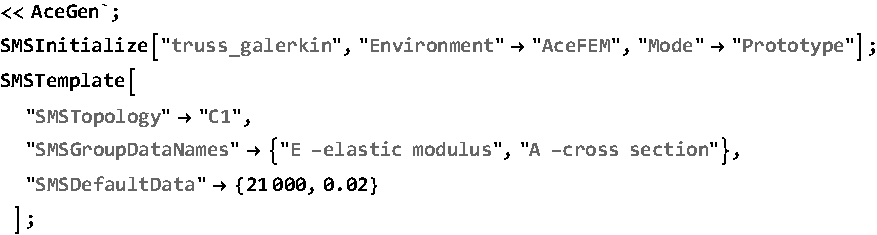
\includegraphics{figures/acegen_input_1}
	\caption{First input}
	\label{fig:first_input}
\end{figure}

Loading the \textit{AceGen} package and initializing constants.


\begin{figure}[htb]
	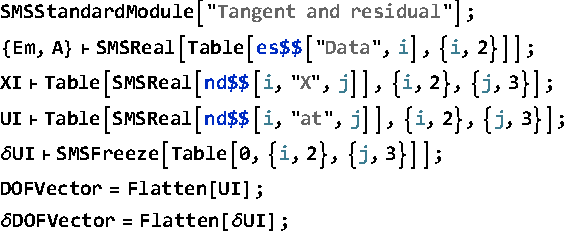
\includegraphics{figures/acegen_input_2}
	\caption{Picking a subroutine and defining variables}
	\label{fig:subroutine}
\end{figure}

\textit{nd\$\$} denotes the nodal data, and \textit{es\$\$} denotes the element structure.
The initialized variational quantities only find use in the standard Galerkin Method.  

\begin{figure}[htb]
	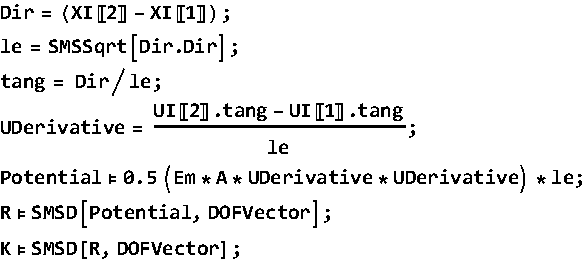
\includegraphics{figures/potentialcode}
	\caption{Main Code for the Potential}
	\label{fig:potential}
\end{figure}
Figure (\ref{fig:potential}) shows the constitutive law, vector \textbf{R}, and matrix \textbf{K}.

\clearpage

\begin{figure}[htb]
	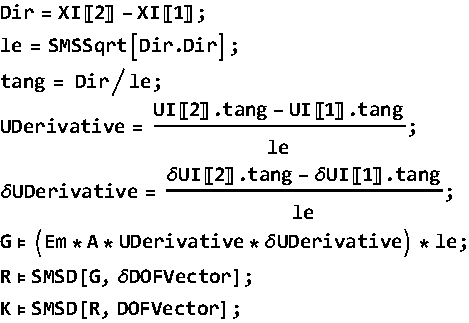
\includegraphics{figures/galerkincode}
	\caption{Main Code for the Standard Galerkin Method}
	\label{fig:galerkin}
\end{figure}

The Standard Galerkin Method uses variational quantities or \textit{trial functions}.

\begin{figure}[htb]
	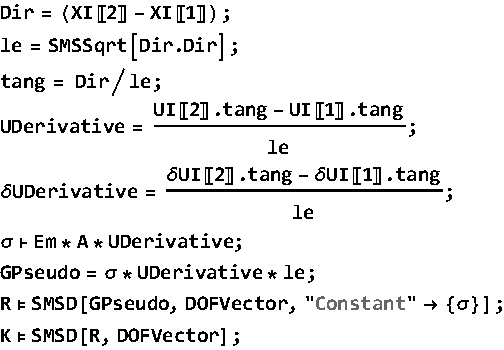
\includegraphics{figures/pseudopotcode}
	\caption{Main Code for the Pseudo Potential}
	\label{fig:pseudo_potential}
\end{figure}

In the Pseudo Potential, a differentiation exception as mentioned in (\ref{eq:pseudoexception}) is used.

\begin{figure}[htb]
	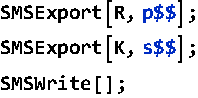
\includegraphics{figures/acegen_input_4}
	\caption{Export}
	\label{fig:Export}
\end{figure}

Lastly, the element is finalized and the element matrices \textbf{R} and \textbf{K} are exported to the fields \textit{p\$\$}, the element load vector, and \textit{s\$\$}, the element stiffness matrix, in \textit{AceFEM}.

\newpage
\section{AceFEM examples}

\begin{figure}[htb]
	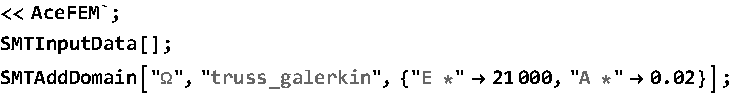
\includegraphics{figures/acefem_input_0}
	\caption{AceFEM system}
	\label{fig:AceFEM First Steps}
\end{figure}

\textit{AceFEM} is initialized and a domain is created. 

\begin{figure}[htb]
	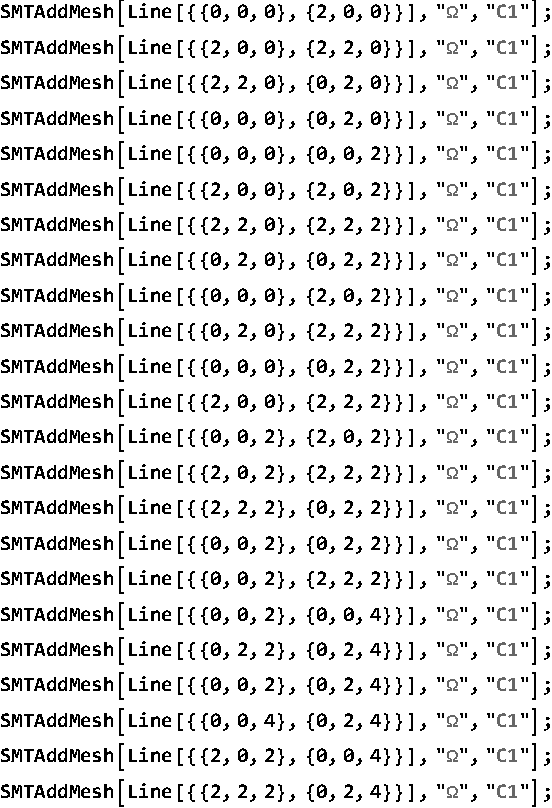
\includegraphics{figures/acefem_input_1}
	\caption{AceFEM system}
	\label{fig:Meshing}
\end{figure}

This mesh is done manually by generating lines with the given element type \textit{C1} on domain \textit{$\Omega$}. A visual example is provided in Figures (\ref{fig:mesh}) and (\ref{fig:def_mesh}).
\clearpage

\begin{figure}[htb]
	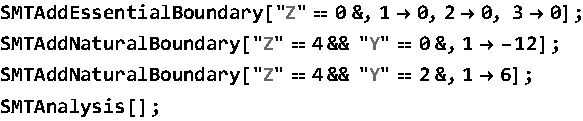
\includegraphics{figures/acefem_input_2}
	\caption{Boundary Conditions And Calculus Phase}
	\label{fig:bound}
\end{figure}

Boundary conditions are applied where necessary, and \textit{AceFEM} is tasked to proceed to calculations.

\begin{figure}[htb]
	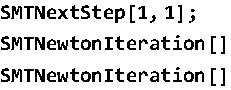
\includegraphics{figures/acefem_input_3}
	\caption{The Last Input: Newton Iterations }
	\label{fig:newton}
\end{figure}

The problem is analyzed by setting the load factor to one, and performing two Newton steps, which is sufficient for a linear problem.

\begin{figure}
	\begin{subfigure}[b]{0.4\textwidth}
		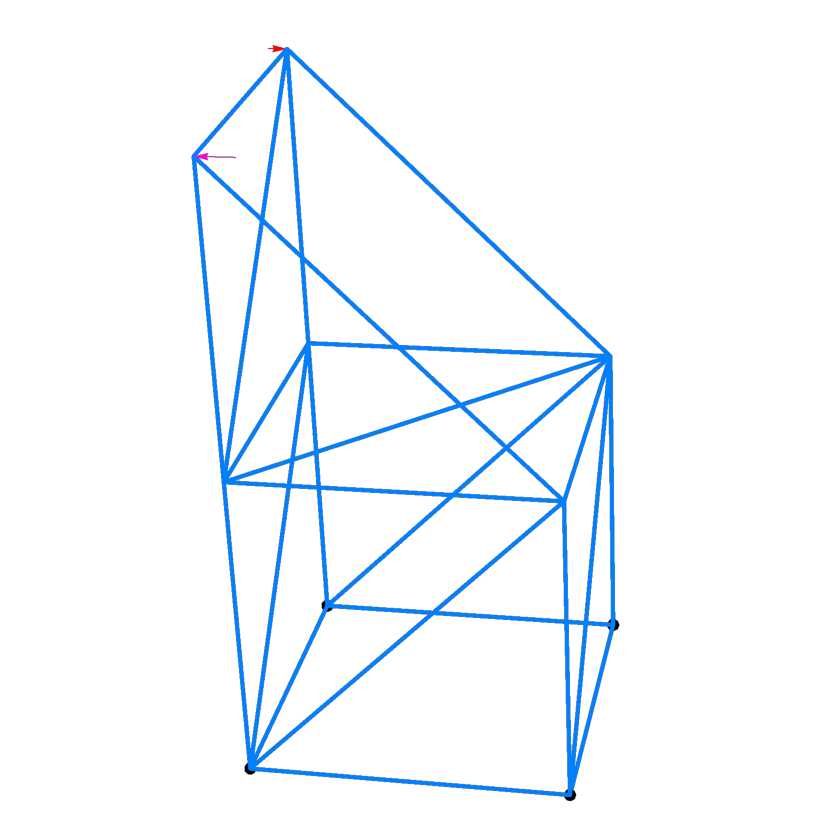
\includegraphics[width=\textwidth]{figures/undeformed}
		\caption{Undeformed mesh}
		\label{fig:mesh}
	\end{subfigure}
	%
	\begin{subfigure}[b]{0.4\textwidth}
		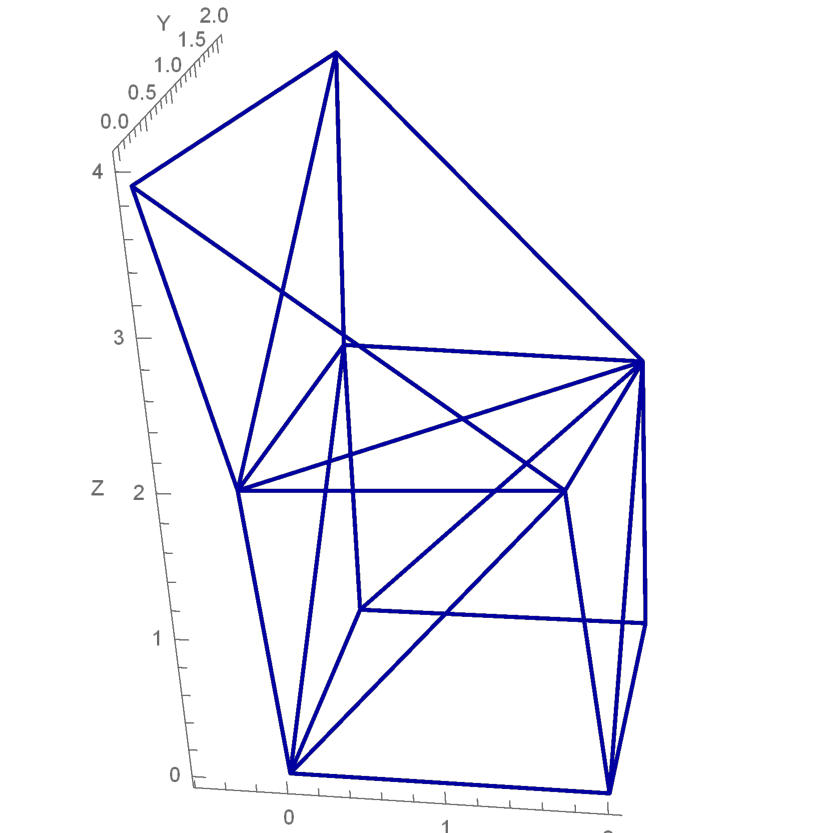
\includegraphics[width=\textwidth]{figures/deformed}
		\caption{Deformed mesh}
		\label{fig:def_mesh}
	\end{subfigure}
	\\ \vspace{5mm}The 2 Figures above show the results of the aforementioned code.
	
\end{figure}




%\include{} 
% ------- layout-datei --------------
\bibliographystyle{plainnat}
%\bibliographystyle{plaindin}
%\bibliographystyle{plaindin_shortname2}
%\bibliographystyle{elsarticle-num-names}
% ------- bib-datei --------------
%\bibliography{bibliography/bibfile01}
%\begin{appendix}

%\end{appendix}
\end{document}
-